Un parametro utile ad indicare quanto un dispositivo MOSFET possa regolare la corrente di drain $I_D$, tramite la tensione $V_{GS}$, è la transconduttanza $g_m$. La quale è definita dal rapporto incrementale:

$$g_m = \frac{\partial I_D}{\partial V_{GS}}$$

Nel caso di $I_D-V_{GS}$ in regione lineare, si ottiene l'espressione:

$$g_m = \frac{W}{L} \cdot \mu \cdot C_{ox} \cdot (V_{GS} - V_{th})$$


\todo[inline]{Da aggiungere cose ho scritto troppo poco}

A figura \ref{fig:gm_w} vengono mostrati i grafici relativi alla transconduttanza per i diversi transistori MOSFET, sia a canale N che P.  

\begin{figure}[ht]
    \centering
    % W = 100 
    \includegraphics[width=0.49\textwidth]{./capitolo2/transconduttanza/gm/NMOS/gm_w_100_vds_900_mV.png}
    \includegraphics[width=0.49\textwidth]{./capitolo2/transconduttanza/gm/PMOS/gm_w_100_vds_900_mV.png}

    \vspace{0.5cm}
    % W = 200
    \includegraphics[width=0.49\textwidth]{./capitolo2/transconduttanza/gm/NMOS/gm_w_200_vds_900_mV.png}
    \includegraphics[width=0.49\textwidth]{./capitolo2/transconduttanza/gm/PMOS/gm_w_200_vds_900_mV.png}
    % W = 600
    \vspace{0.5cm}

    \includegraphics[width=0.49\textwidth]{./capitolo2/transconduttanza/gm/NMOS/gm_w_600_vds_900_mV.png}
    \includegraphics[width=0.49\textwidth]{./capitolo2/transconduttanza/gm/PMOS/gm_w_600_vds_900_mV.png}

    \caption{Transconduttanza calcolata nei dispositivi MOSFET prima di subire la dose di irraggiamento. canale N, a sinistra, e canale P, a destra, i grafici sono raggruppati per larghezza di canale.}
    \label{fig:gm_w}

\end{figure}


\todo[inline]{Al momento metto i grafici}

\begin{figure}[ht]
    \centering
    % W = 100 
    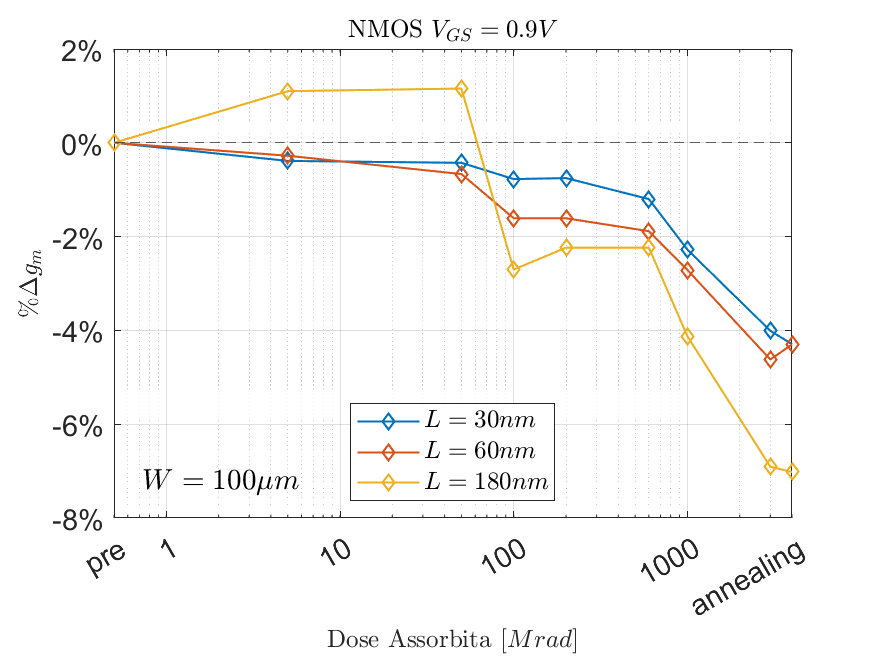
\includegraphics[width=0.49\textwidth]{./capitolo2/transconduttanza/delta_gm_N/vds_0_9/Delta_Gm_NMOS_Vds_0_9_W_100.png}
    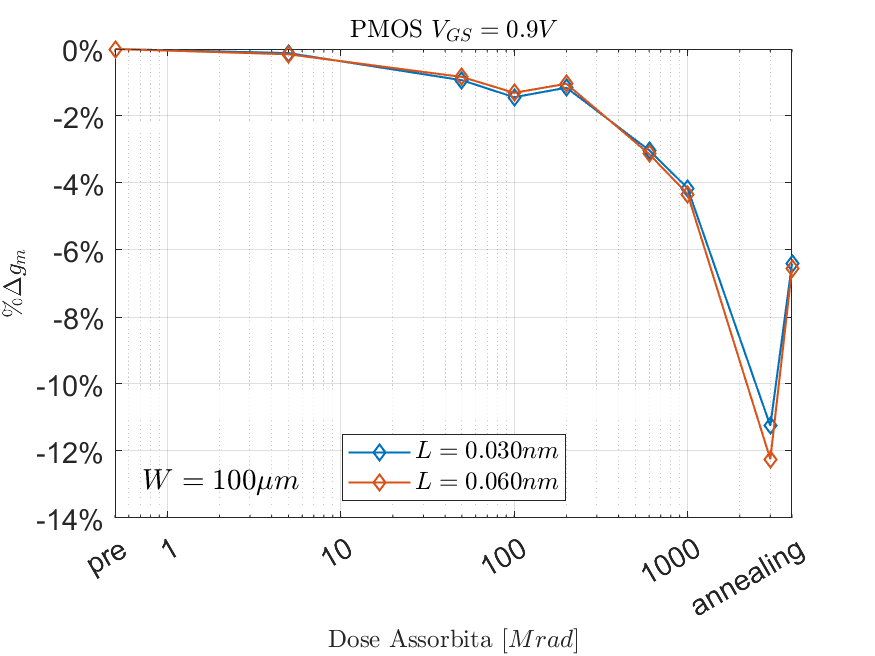
\includegraphics[width=0.49\textwidth]{./capitolo2/transconduttanza/delta_gm_P/vds_0_9/Delta_Gm_PMOS_Vds_0_9_W_100.png}

    \vspace{0.5cm}
    % W = 200
    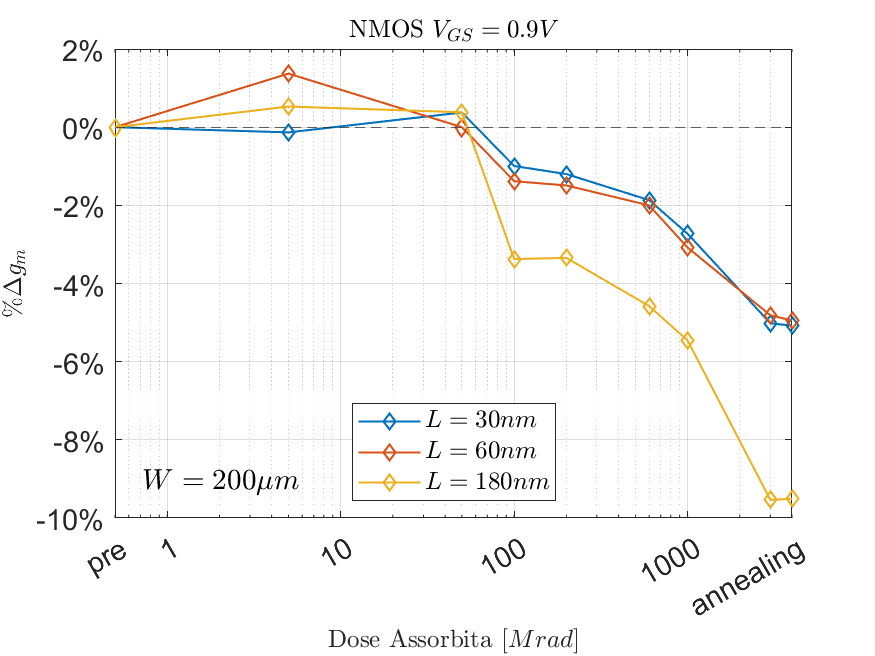
\includegraphics[width=0.49\textwidth]{./capitolo2/transconduttanza/delta_gm_N/vds_0_9/Delta_Gm_NMOS_Vds_0_9_W_200.png}
    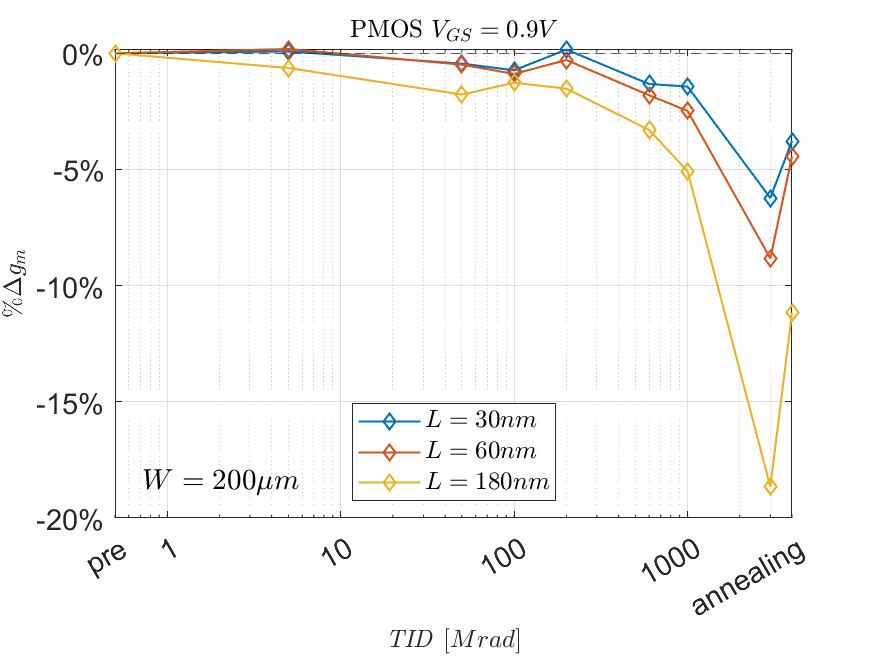
\includegraphics[width=0.49\textwidth]{./capitolo2/transconduttanza/delta_gm_P/vds_0_9/Delta_Gm_PMOS_Vds_0_9_W_200.png}
    % W = 600
    \vspace{0.5cm}

    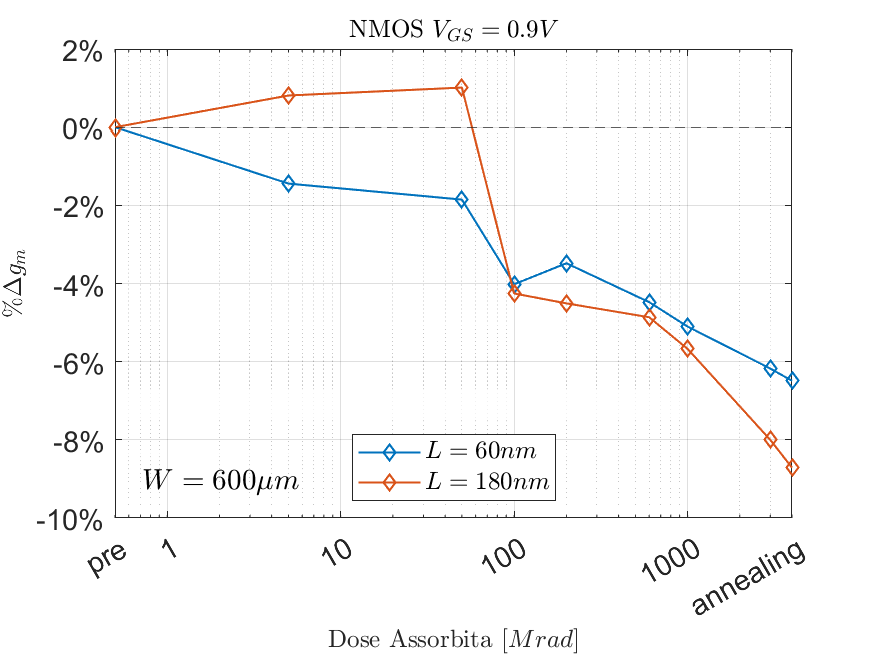
\includegraphics[width=0.49\textwidth]{./capitolo2/transconduttanza/delta_gm_N/vds_0_9/Delta_Gm_NMOS_Vds_0_9_W_600.png}
    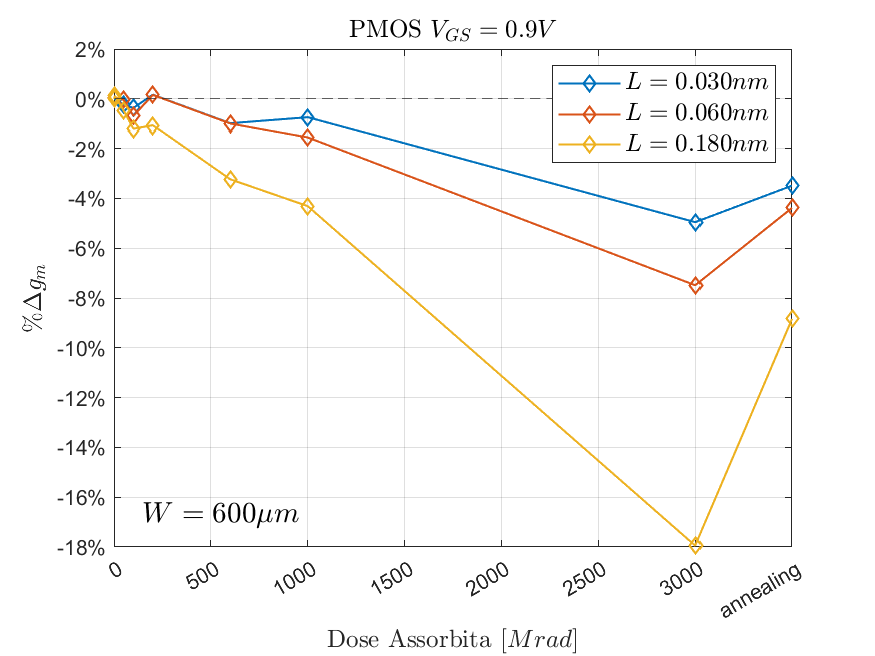
\includegraphics[width=0.49\textwidth]{./capitolo2/transconduttanza/delta_gm_P/vds_0_9/Delta_Gm_PMOS_Vds_0_9_W_600.png}
    \caption{Curve $\Delta g_m $ percentuale al variare della dose assorbita: a sinistra i transistori MOSFET a canale N e a destra a canale P. I grafici sono raggruppati per larghezza di canale.}
    \label{fig:delta_gm}


\end{figure}

